%%%%%%%%%%%%%%%%%%%%%%%%%%%%%%%%%%%%%%%%%%%%%%%%%%%%%%%%
%   |------------------------------------------|       %
%   | Web App embebida en dispositivos móviles |       %
%   |  para la gestión de registros sobre la   |       %
%   |   contaminación de afluentes y ríos.     |       %
%   |                                          |       %
%   |          Proyecto de graduación          |       %
%   |__________________________________________|       %
%                                                      %
%   Autores                                            %
%   -------                                            %
%                                                      %
% * Bruno, Ricardo Hugo (CX 1409686)                   %
%     rburnount@gmail.com                              %
% * Gómez Veliz, Kevin Shionen (CX 1411828)            %
%     ing.gomezvelizkevin@gmail.com                    %
%                                                      %
%   Tutor                                              %
%   -------                                            %
%                                                      %
% * Ing. Cohen, Daniel Eduardo                         %
%        dcohen.tuc@gmail.com                          %
%                                                      %
%   Cotutor                                            %
%   -------                                            %
%                                                      %
% * Ing. Nieto, Luis Eduardo                           %
%        lnieto@herrera.unt.edu.ar                     %
%                                                      %
%                                                      %
%%%%%%%%%%%%%%%%%%%%%%%%%%%%%%%%%%%%%%%%%%%%%%%%%%%%%%%%

\chapter{Disciplina de Implementación}
\label{chap:implementacion}

\section{Diagrama conceptual estructura Cliente/Servidor/Internet}
    \begin{figure}[H]
        \centering
        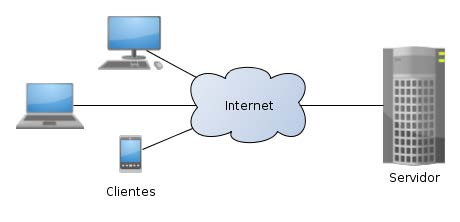
\includegraphics[width=1\textwidth]{imagenes/implementacion/clienteServidorInternet.jpg}
        \label{clienteServidorInternet}
    \end{figure}


\section{Arquitectura de la aplicación}

\begin{figure}[H]
  \centering
    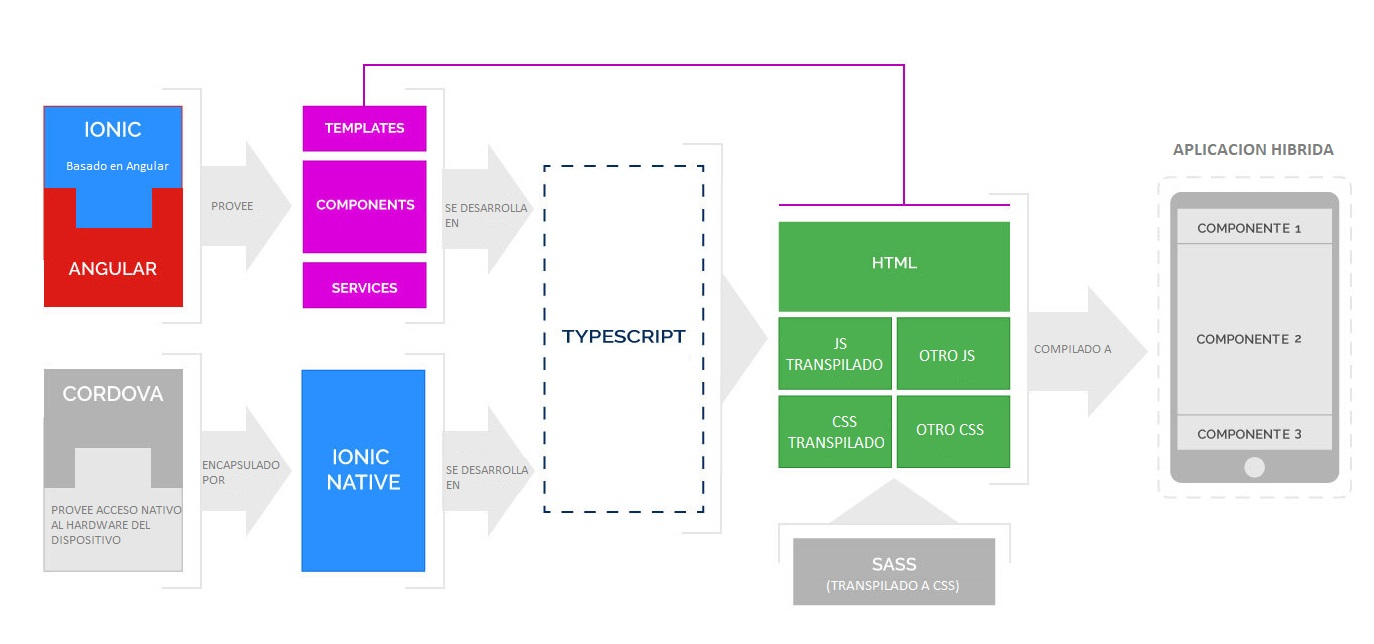
\includegraphics[width=1\textwidth]{imagenes/implementacion/interfazDeUsuario.jpg}
    
     \caption{Interfaz de Usuario}
    \label{fig:arquitectura-aplicacion}
\end{figure}

    \begin{figure}[H]
        \centering
        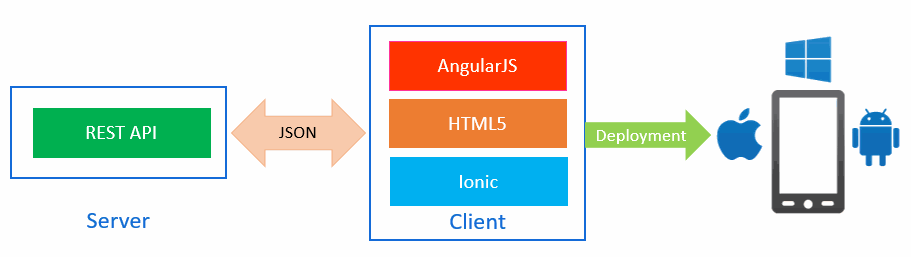
\includegraphics[width=1\textwidth]{imagenes/implementacion/despliegue.png}
        \caption{Diagrama de Despliegue}
        \label{diagrama-despliegue}
    \end{figure}


\section{Modelo-Vista-Controlador}

Modelo-Vista-Controlador (en adelante MVC) es un patrón de diseño que permite
separar la capa de datos y lógica de negocios (modelos y controladores), de la interfaz
de usuario (vista).

\subsection{Componentes del patrón}
\begin{itemize}
    \item \textbf{Modelo}: Es la representación de la información con la cual el sistema opera. Se
    puede pensar en un modelo como una tabla en el sistema gestor de bases de datos.
    Si bien este enfoque resulta sumamente útil para trabajar con el patrón MVC,
    el modelo también requiere de funcionalidades que faciliten la interacción con los
    demás controladores, vistas y modelos del sistema.
    \item \textbf{Vista}: Es la representación gráfica de los datos. Provee la interfaz mediante la cual
    los usuarios realizan la entrada de los datos y observan el resultado del procesamiento
    de dichos datos.
    \item \textbf{Controlador}: Sirve como nexo entre las vistas y los modelos. El controlador responde
    usualmente a eventos que son generados por el usuario en su interacción con
    la vista. La vista brinda al usuario un mecanismo para comunicarse con un controlador,
    y es este ultimo el encargado de obtener los datos ingresados por el usuario,
    pasarlos al modelo adecuado para su procesamiento, recibir la salida del modelo y
    enviar dicha salida a la vista para su visualización.
    
\end{itemize}



\section{Elección del Lenguaje}

    Independientemente del paradigma de ingeniería de software, el lenguaje de programación tendrá impacto en la planificación, el análisis, el diseño, la codificación, la prueba y el mantenimiento de un proyecto. Para la construcción de la aplicación se eligió la utilización de los lenguajes web HTML5, CSS3 y JavaScript.

    La elección de estos lenguajes para la construcción de la aplicación se debe a las siguientes ventajas que ofrecen:
    \begin{itemize}
        \item \emph{Mayor portabilidad:} Al ser tecnologías estándares y soportadas por la mayoría de los teléfonos celulares modernos, es posible que una misma aplicación sea muy fácilmente adaptable a varias plataformas móviles.
        \item \emph{Soporte futuro:} Todas las plataformas móviles están trabajando para mejorar el soporte que ofrecen a las tecnologías web, ofreciendo una mejor experiencia al usuario.
        \item \emph{Aprovechamiento de conocimiento de desarrollo de aplicaciones web:} Desarrollando aplicaciones móviles en \gls{HTML}5, \gls{CSS}3 y \gls{JavaScript} es posible aplicar el conocimiento en el desarrollo de aplicaciones web desarrolladas para navegadores en equipos de escritorio 
    \end{itemize}

\section{Apache Cordova}

\begin{figure}[H]
  \centering
    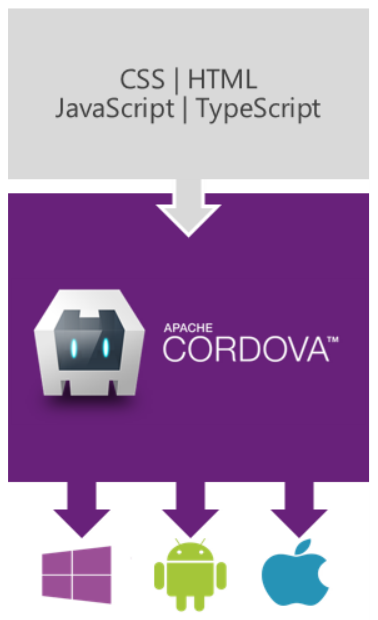
\includegraphics[width=0.5\textwidth]{imagenes/cordova-architecture.png}
    
     \caption{Arquitectura de Apache Cordova}
    \label{arquitectura-Apache Cordova}
\end{figure}

Apache Cordova es un \gls{framework} de código abierto que actúa como un intermediario entre las aplicaciones web y los dispositivos móviles. Permite crear aplicaciones móviles listas para instalar utilizando tecnología web: \gls{JavaScript}, \gls{HTML}5 y \gls{CSS}3.

Las aplicaciones resultantes no son totalmente nativas, ni puramente basado en la web. La desventaja de que una aplicación sea totalmente nativa es que solo se podrá utilizar para la plataforma para la que fue realizada, es decir si se hace una aplicación para Android luego no se podrá reutilizar el código para hacer la misma aplicación para iOS.

Con Apache Cordova se puede reutilizar el código de una aplicación para crear el paquete instalador de cualquiera de las 7 plataformas móviles soportadas: iOS, Android, Blackberry, Windows Phone, WebOS de Palm, Symbian, Bada, entre otras.

Apache Cordova permite acceder a funciones nativas como el acelerómetro, cámara, brújula, contactos, archivos, ubicación geográfica, almacenamiento  y notificaciones.

\subsection{Ventajas de Apache Cordova}

\begin{itemize}

    \item Soporte multiplataforma
    
    \item Acceso a características nativas de cada plataforma a través de su API, a las que una aplicación web visitada desde el navegador no podría acceder, como acceso a la cámara de fotos, acelerómetro, notificaciones, etc.
    
    \item Permite ejecutar a través de JavaScript plugins escritos en código nativo.
    
    \item Permite distribuir aplicaciones realizadas utilizando HTML5 y JavaScript a través de las tiendas de aplicaciones oficiales de cada plataforma.
    
    \end{itemize}
    \subsection{Desventaja de Apache Cordova}
    \begin{itemize}
\item Normalmente las aplicaciones realizadas con Apache Cordova tienen un menor rendimiento en tareas que requieren alta capacidad de procesamiento, sobre todo en versiones antiguas de las plataformas sobre las que se usa.

\item Se pierde la posibilidad de acceder a algunas características nativas, como los diferentes elementos de interfaz de usuario propios de cada plataforma, aunque estos pueden imitarse mediante el uso de CSS.
\end{itemize}

\section{Web services}
\label{sec:webservices}

Un servicio web (en inglés, Web service) es una tecnología que utiliza un conjunto de protocolos y estándares que sirven para intercambiar datos entre aplicaciones. Distintas aplicaciones de software desarrolladas en lenguajes de programación diferentes, y ejecutadas sobre cualquier plataforma, pueden utilizar los servicios web para intercambiar datos en redes de ordenadores como Internet. La interoperabilidad se consigue mediante la adopción de estándares abiertos.

Las ventajas de los servicios web son:

\begin{itemize}
    \item Aportan interoperabilidad entre aplicaciones de software independientemente de sus propiedades o de las plataformas sobre las que se instalen.
    \item Los servicios Web fomentan los estándares y protocolos basados en texto, que hacen más fácil acceder a su contenido y entender su funcionamiento.
    \item Permiten que servicios y software de diferentes compañías ubicadas en diferentes lugares geográficos puedan ser combinados fácilmente para proveer servicios integrados.
   
 \end{itemize}
 
\subsection{Razones para crear servicios Web}

La principal razón para usar servicios Web es que se pueden utilizar con HTTPS sobre \gls{TCP} en el puerto 443. Dado que las organizaciones protegen sus redes mediante firewalls -que filtran y bloquean gran parte del tráfico de Internet, cierran casi todos los puertos TCP salvo el 443, que es, precisamente, el que usan los navegadores. Los servicios Web utilizan este puerto, por la simple razón de que no resultan bloqueados. Es importante señalar que los servicios web se pueden utilizar sobre cualquier protocolo, sin embargo, TCP es el más común.

Otra razón por la que los servicios Web son muy prácticos es que pueden aportar gran independencia entre la aplicación que usa el servicio Web y el propio servicio. De esta forma, los cambios a lo largo del tiempo en uno no deben afectar al otro. Esta flexibilidad será cada vez más importante, dado que la tendencia a construir grandes aplicaciones a partir de componentes distribuidos más pequeños es cada día más utilizada.
Se pueden desarrollar servicios web como parte de una aplicación web, permitiendo acceder a los mismos datos que esta.


\subsection{REST}

REST es una técnica de arquitectura software para sistemas hipermedia distribuidos como la World Wide Web.
Los sistemas que siguen los principios REST se llaman con frecuencia RESTful.

\begin{figure}[htbp]
  \centering
    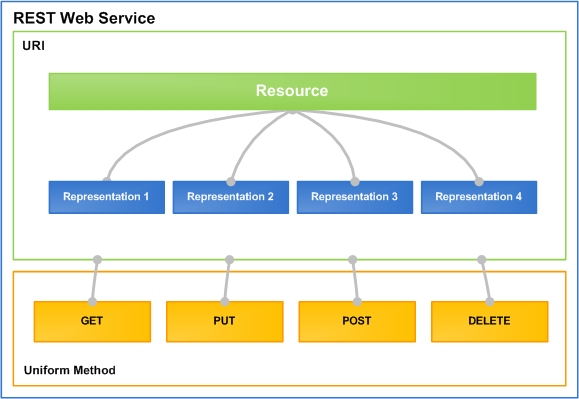
\includegraphics[width=0.8\textwidth]{imagenes/REST.jpg}
     \caption{Web Services REST}
    \label{fig:REST}
\end{figure}

REST afirma que la web ha disfrutado de escalabilidad como resultado de una serie de diseños fundamentales clave:

\begin{itemize}
    \item \emph{Un protocolo cliente/servidor sin estado:} cada mensaje HTTP contiene toda la información necesaria para comprender la petición. Como resultado, ni el cliente ni el servidor necesitan recordar ningún estado de las comunicaciones entre mensajes. Sin embargo, en la práctica, muchas aplicaciones basadas en HTTP utilizan cookies y otros mecanismos para mantener el estado de la sesión (algunas de estas prácticas, como la re escritura de URLs, no son permitidas por REST)
    
    \item \emph{Un conjunto de operaciones bien definidas que se aplican a todos los recursos de información:} HTTP en sí define un conjunto pequeño de operaciones, las más importantes son POST, GET, PUT y DELETE.
    
    \item Una sintaxis universal para identificar los recursos. En un sistema REST, cada recurso es direccionable únicamente a través de su \gls{URI}.
   
 \end{itemize}
 
 \subsubsection{Recursos}
 Un concepto importante en REST es la existencia de recursos (elementos de información), que pueden ser accedidos utilizando un identificador global (un Identificador Uniforme de Recurso).
 
 Para manipular estos recursos, los componentes de la red (clientes y servidores) se comunican a través de una interfaz estándar (HTTP) e intercambian representaciones de estos recursos (los ficheros que se descargan y se envían.
 
\section{Express.js}

Express es una infraestructura de aplicaciones web Node.js mínima y flexible que proporciona un conjunto sólido de características para las aplicaciones web y móviles.
Con miles de métodos de programa de utilidad HTTP y middleware a su disposición, la creación de una API sólida es rápida y sencilla.
Express proporciona una delgada capa de características de aplicación web básicas, que no ocultan las características de Node.js.

\section{Herramientas de desarrollo}

\begin{itemize}

\item \emph {Visual Code:} Visual Studio Code es un editor de código fuente desarrollado por Microsoft para Windows , Linux y macOS. Incluye soporte para la depuración, control integrado de Git. Es gratuito y de código abierto.

\item \emph {Draw.io:} Es un stack de tecnología de código abierto para crear aplicaciones de diagramación, entre ellas UML.
Permite dibujar todos los tipos de diagramas de clases, código inverso, generar código desde diagramas y generar documentación.

\item \emph{\LaTeX:} Es un sistema de composición de textos, orientado especialmente a la creación de libros, documentos científicos y técnicos que contengan fórmulas matemáticas.

\LaTeX facilita el uso del lenguaje de composición tipográfica. Es muy utilizado para la composición de artículos académicos, tesis y libros técnicos, dado que la calidad tipográfica de los documentos realizados con \LaTeX es comparable a la de una editorial científica de primera línea.

\item \emph{GitHub:} Es una forja (plataforma de desarrollo colaborativo) para alojar proyectos utilizando el sistema de control de versiones Git. Se utiliza principalmente para la creación de código fuente de programas de computadora.

\end{itemize}

\section{Persistencia de clases}

    \subsection{Modelo físico del sistema}
        En esta actividad se define la estructura física de los datos utilizada en el sistema. 
        Este esquema contempla las maneras de acceder físicamente a los datos, por medio de claves, índices, etc., para cumplir todos los requisitos. 
        En esta fase se tienen que tener en cuenta aspectos de funcionalidad y rendimiento en el funcionamiento de la aplicación. Es decir, se modificara el diseño lógico de datos, para convertirlo en un modelo físico, que contemple todas estos aspectos de funcionalidad y rendimiento. Se comentaran de manera individualiza el porque de cada una de las modificaciones realizadas en el modelo físico, justificando su ejecución.

		\subsection{Modelo relacional. Vista de la base de datos}
			\begin{figure}[H]
				\centering
				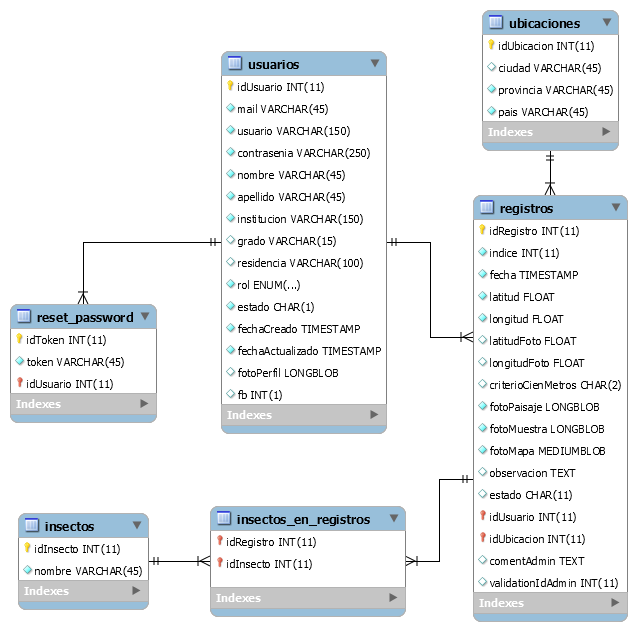
\includegraphics[width=1\textwidth]{imagenes/implementacion/db.png}
				\caption{Modelo completo}
				\label{diagrama-despliegue}
			\end{figure}